\documentclass[a4paper, 11pt]{article}
\usepackage[utf8]{inputenc}
\usepackage[T1]{fontenc}
%\usepackage[ngerman,english]{babel}

\usepackage{amsmath}
\usepackage{commath}
\usepackage{textcomp}
\usepackage[squaren,thinspace,thinqspace]{SIunits}
\usepackage[minionint, lf]{MinionPro}
\usepackage[medfamily, sansmath, lf]{MyriadPro}
\usepackage[usenames,dvipsnames]{xcolor}
\usepackage{soul}

\usepackage{tikz}
\usetikzlibrary{arrows,shapes,positioning,shadows,trees}

\usepackage{microtype}
\usepackage{graphicx}
\usepackage{lipsum}
%\usepackage[normalem]{ulem}
\usepackage[round]{natbib}
\usepackage{titlesec}
\usepackage{geometry}
\usepackage{verbments}
\usepackage{minted}
\usepackage{multicol}
\usepackage[font=small,labelfont=bf]{caption}
\usepackage{subcaption}
\usepackage{booktabs}
\usepackage[title]{appendix}

\usepackage{pifont}
\newcommand{\cmark}{\ding{51}}%
\newcommand{\xmark}{\ding{55}}%

% Package that provides hyperlinks to (in this case) citations
\usepackage[pdfauthor={Patrick Camilleri},
pdftitle={Fault tolerance mechanism implementations in SpiNNaker},
pdfsubject={Fault tolerance},
pdfkeywords={faulttolerance spinnaker}
]{hyperref} % This loads package 'url'

\hypersetup{colorlinks=true,
	citecolor=Sepia,
	urlcolor=blue,
	filecolor=black,
	linkcolor=black,
	breaklinks=true}
\urlstyle{same}

\usepackage{geometry}
\geometry{
	a4paper,
	total={210mm,297mm},
	left=35mm,
	right=30mm,
	top=30mm,
	bottom=30mm,
}

\newenvironment{itmz}{
	\begin{itemize}
		\setlength{\itemsep}{0pt}
		\setlength{\parskip}{0pt}
	}{\end{itemize}}

\tikzset{
	treenode/.style = {align=center, inner sep=3pt, text centered},
	arn/.style = {treenode, rectangle, draw=black, rounded corners=4pt, fill=blue!20, font=\sffamily\bfseries, text width=10em},
	arn_lev1/.style = {treenode, text width=6em},
	arn_lev2/.style = {treenode, text width=6em},
	arn_lev2a/.style = {treenode, text width=5.8em}
}

% Fancy title page
\makeatletter
\newlength\drop
\newcommand*{\titleGM}{%
\thispagestyle{empty}
\begingroup% Gentle Madness
\drop = 0.1\textheight
\vspace*{\baselineskip}
\vfill
\hbox{%
  \hspace*{0.2\textwidth}%
  \rule{1pt}{\dimexpr\textheight-28pt\relax}%
  \hspace*{0.05\textwidth}% 
  \parbox[b]{0.75\textwidth}{%
    \vbox{%
      \vspace{\drop}
      {\Huge\bfseries\raggedright\@title\par}\vskip2.37\baselineskip
      {\Large\itshape PRiME Project }\\[4\baselineskip]
      {\Large\bfseries\@author\par}
      \vspace{0.5\textheight}
    }% end of vbox
  }% end of parbox
}% end of hbox
\vfill
\cleardoublepage % this clears the page number from the second (empty) title page
\null % this creates a second blank page (with page number)
\endgroup}
\makeatother

\setcounter{secnumdepth}{4}
\setcounter{tocdepth}{3}

\title{Fault tolerance mechanism implementations in SpiNNaker}
\author{Patrick Camilleri}
\date{}

\begin{document}
\maketitle

\tableofcontents

\newpage
\section{Software fault tolerance}
\label{sec:software_ft}

\subsection{Introduction}
This report will first outline (\textbf{Section~\ref{sec:software_ft}}) some fault tolerance basics and concepts from the field of software fault tolerance \citep{trivedi2008software} with the hope that the some of the ideas can be extended to SpiNNaker, a massively parallel processing machine. \textbf{Section~\ref{sec:ft_spinnaker}} details the various hardware blocks in the SpiNNaker chip which provide features that could be used to implement fault tolerant mechanisms to benefit the system as a whole. \textbf{Sections \ref{sec:congestion}} and~\textbf{\ref{sec:migration}} show some working examples of how fault tolerance is currently being implemented in SpiNNaker and \textbf{Section~\ref{sec:crc}} outlines the properties of the CRC unit implemented in SpiNNaker and suggestions by \citet{grymel2013error} of how to perform 1-bit error correction when doing DMA transfers.

While hardware failures have been studied extensively and varied mechanisms have been presented to increase the system availability with regard to such failures, software failures and the corresponding reliability/availability analysis has not drawn much attention from researchers. The study of software failures has now become more important since it has been recognized that computer systems outages are more due to software faults than to hardware faults \citep{gray1991high}. For a long time it was assumed that concepts of reliability and failure rate do not apply to software since software does not degrade physically as a function of time or environmental conditions. Many studies have shown that even for applications which have relatively less complex software, many failures in computer systems are due to software bugs \citep{pradhan1996fault}. Therefore, software reliability is one of the weakest links in system reliability.

Present-day applications have strict reliability and availability demands, because in many cases there are serious consequences like huge economic losses or risk to human life if the software is faulty. There have been instances of spectacular system failures due to software errors like the crash of the Ariane 5 launcher \citep{lions1996ariane}. Also, increasing complexity and proliferation of real-time software have led to a resultant increase in software failures.

A major limitation in developing reliable software is the test and verification process. Formal verification techniques cannot be applied to large programs. Furthermore, the difficulties in verifying adherence to timing constraints for real-time systems such as SpiNNaker make the software testing and verification process harder. This limitation coupled with the very stringent requirements for fault-free operation of the software form the basis for the need for fault tolerance in software \citep{trivedi2008software}.

\subsection{Classification of Software Faults}
%According to \citet{laprie1992dependability}, ``a system failure occurs when the delivered service no longer complies with the specifications, the latter being an agreed description of the system's expected function and/or service.'' Some studies have suggested that since software is not a physical entity and hence not subject to transient physical phenomena (as opposed to hardware), software faults are permanent in nature \citep{huang1994two}.

Software faults can be classified into hard and soft faults. Hard faults are permanent design faults and hence almost deterministic in nature. They can be identified easily and weeded out during the testing and debugging phase of the software life cycle. Soft faults, on the other hand, belong to the class of temporary internal faults and are intermittent. Hence these faults result in transient failures, i.e., failures which may not recur if the software is restarted. Some typical situations in which intermittent faults might surface are boundaries between various software components, improper or insufficient exception handling and interdependent timing of various events. It is for this reason that intermittent faults are extremely difficult to identify through testing. Most recent studies on failure data have reported that a large proportion of software failures are transient in nature \citep{gray1990census}, caused by phenomena such as overloads or timing and exception errors \citep{chillarege1995measurement}.

\subsection{Techniques for Fault Tolerance in Software}
Means to cope with the existence and manifestation of faults in software can be divided into three main categories:

\begin{itemize}
\item \textbf{Fault avoidance/prevention} includes design methodologies which attempt to make software provably fault-free.
\item \textbf{Fault removal} methods aim to remove faults after the development stage is completed. This is done by exhaustive and rigorous testing of the final product.
\item \textbf{Fault tolerance} makes the assumption that the system has unavoidable and undetectable faults and aims to make provisions for the system to operate correctly even in the presence of faults.
\end{itemize}

Most deterministic and repeatable faults, can be removed through rigorous and extensive testing and debugging, but no amount of testing can certify software as fault-free. The faults remaining after testing and debugging are usually intermittent. Hence, \emph{fault tolerance}, is the only remaining hope to achieve dependable software. Fault tolerance makes it possible for the software system to provide service even in the presence of faults. This means that an imminent failure needs to be prevented or recovered from.

There are two strategies for software fault tolerance: error processing and fault treatment. Error processing aims to remove errors from the software state and can be implemented by substituting an error-free state in place of the erroneous state, or by compensating for the error by providing redundancy, called error compensation. Error recovery can be achieved by either forward or backward error recovery. The second strategy, fault treatment, aims to prevent activation of faults and so action is taken before the error creeps in. \textbf{Figure~\ref{fig:faulttoltree}} shows this classification \citep{trivedi2008software}. Techniques for tolerating faults in software have been divided into three main classes: design diversity, data diversity and environment diversity (see \textbf{Table~\ref{tab:faulttolmethods}}).

\begin{figure}[htbp]
	%\centering
	\hspace*{2cm}
	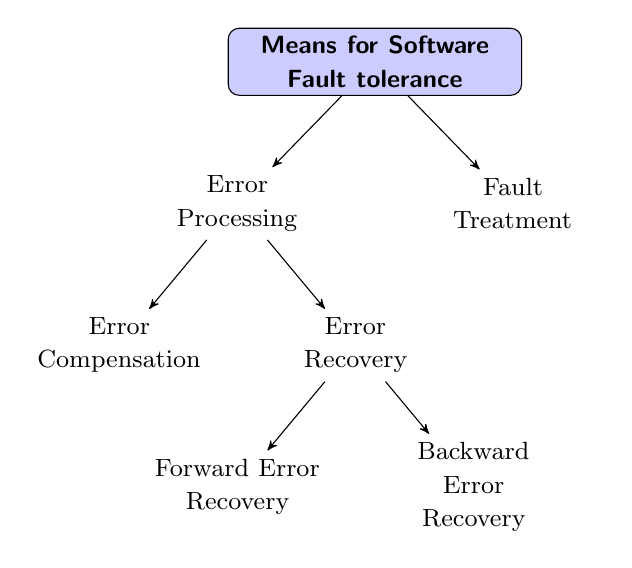
\begin{tikzpicture}[->,>=stealth', 
	level 1/.style={sibling distance = 3.5cm, level distance = 1.8cm},
	level 2/.style={sibling distance = 3cm}
	%	level 3/.style={sibling distance = 3.5cm}
	] 
	\node [arn] {\small Means for Software Fault tolerance}
	child{ node [arn_lev1] {\small Error Processing} 
		child{ node [arn_lev2] {\small Error Compensation} }
		child{ node [arn_lev2] {\small Error Recovery}
			child{ node [arn_lev2] {\small Forward Error Recovery}}
			child{ node [arn_lev2] {\small Backward Error Recovery}}
		}                            
	}
	child{ node [arn_lev1] {\small Fault Treatment} }
	; 
	\end{tikzpicture}
	\caption{Means for software fault tolerance.}
	\label{fig:faulttoltree}
\end{figure}

\begin{table}[h]
	\centering
	\caption{Strategies used by different fault tolerance methods.}
	\label{tab:faulttolmethods}
	\begin{tabular}{l c c c c }
		\toprule
		& Design    & Data      & Environment & Checkpointing \\
		& diversity & diversity & diversity   & \& recovery   \\
		\midrule
		Error compensation & \cmark    & \cmark    &             &               \\
		Error recovery     &           &           &             & \cmark        \\
		Fault treatment    &           &           & \cmark      &               \\
		\bottomrule
	\end{tabular}
\end{table}

\subsubsection{Design diversity}
Design diversity techniques are specifically developed to tolerate design faults in software arising out of wrong specifications and incorrect coding. Two or more variants of a software developed by different teams but to a common specification are used. These variants are then used in a time or space redundant manner to achieve fault tolerance. Popular techniques which are based on the design diversity concept for fault tolerance in software are: N-version programming, recovery block, and N-self checking programming.

\subsubsection{Data diversity}
\citet{ammann1988data} introduced the data diversity technique for fault tolerance. While the design diversity approaches to provide fault tolerance rely on multiple versions of the software written to the same specifications, the data diversity approach uses only one version of the software. This approach relies on the observation that a software sometime fails for certain values in the input space and this failure could be averted if there is a minor perturbation of input data which is acceptable to the software. N-copy programming, based on data diversity, has N copies of a program executing in parallel, but each copy running on a different input set produced by a diverse-data system. The diverse-data system produces a related set of points in the data space. Selection of the system output is done using an enhanced voting scheme which may not be a majority voting mechanism. In some cases like a real-time control program, a minor perturbation in sensor values may be able to prevent a failure since sensor values are usually noisy and inaccurate. Data diversity can work well with permanent faults and is cheaper to implement than design diversity techniques. To some extent, data diversity can also deal with intermittent faults since different input data is presented and by definition, these bugs are non-deterministic and non-repeatable \citep{kapur2011software}.

\subsubsection{Environment diversity}
\label{sec:envdiv}
Environment diversity is the newest approach to fault tolerance in software. Although this technique has been used for long in an ad hoc manner, only recently has it gained recognition and importance. Having its basis on the observation that most software failures are transient in nature, the environment diversity approach requires re-executing the software in a different environment \citep{jalote1995framework}. Environment diversity deals effectively with intermittent faults by exploiting their definition and nature.

\citet{adams1984optimizing} has proposed restarting the system as the best approach to masking software faults. Transient faults typically occur in computer systems due to design faults in software which result in unacceptable and erroneous states in the operating system environment. Therefore environment diversity attempts to provide a new or modified operating environment for the running software. Usually, this is done at the instance of a failure in the software. When the software fails, it is restarted in a different, error-free state which is achieved by some clean up operations. Examples of environment diversity techniques include retry operation, restart application and rebooting the node. The retry and restart operations can be done on the same node or on a spare node.

\subsubsection{Checkpointing and recovery}
Checkpointing and recovery \citep{kulkarni1990effects} belongs to the category of error recovery for fault tolerance, as opposed to design diversity which belongs to error compensation, and data and environment diversities which belong to the fault treatment category. Error compensation, error recovery and fault treatment are complementary to one another and fault tolerance in software can be increased by deploying a combination of these techniques. The recovery block uses checkpoints in its implementation. \citet{garg1996minimizing} proposes and analyses the combination of software rejuvenation (preventive fault treatment) with checkpointing and recovery to reduce the chances of activating a fault and simultaneously minimizing the loss of computation when there is a failure.

Checkpointing involves occasionally saving the state of a process in stable storage during normal execution. Upon failure, the process is restarted in the saved state (last saved checkpoint). Checkpointing and recovery was mainly intended to tolerate transient hardware failures, where the application is restarted upon repair of a hardware unit after failure. This technique has been implemented in both software and hardware.

\newpage
\section{Fault tolerance in SpiNNaker}
\label{sec:ft_spinnaker}

With regards to the PRiME project the issue of fault tolerance is being currently investigated on the SpiNNaker platform while always keeping in view the issue of power reduction and optimisation. The three main fault-tolerant mechanisms that are being investigated are:
\begin{itemize}
\item Dropped packet re-insertion,
\item Function/Process migration,
\item CRC error detection/correction of SDRAM blocks.
\end{itemize}
More in-depth information and experimental results will be presented in the following sections. But first, an overview of the SpiNNaker architecture as well the various fault tolerance mechanisms at the disposal of the low-level system programmer available on the SpiNNaker chip will be presented.

\subsection{SpiNNaker architecture}

The SpiNNaker engine is a massively-parallel multi-core computing system. The final machine will contain up to approximately one million ARM9 cores and 7~TB of RAM distributed throughout the system in 57,000 nodes, each node being a System-in-Package (SiP) containing 18 cores plus a 128~MB off-die SDRAM (Synchronous Dynamic Random Access Memory). Each core has associated with it 64~kB of data tightly-coupled memory (DTCM) and 32~kB of instruction tightly-coupled memory (ITCM). The cores have a variety of ways of communicating with each other and with the memory, the dominant of which is by packets. These are 5- or 9-byte (40- or 72-bit) quanta of information that are transmitted around the system with the help of a concurrent hardware routing system. 

\begin{figure}[htbp]
	\centering
	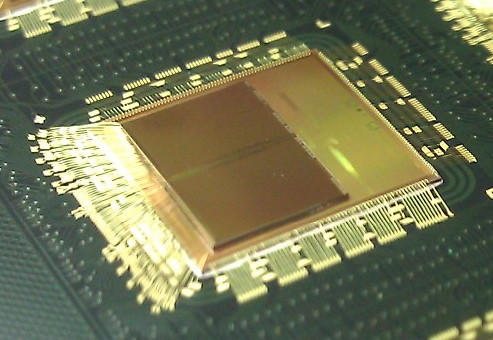
\includegraphics[width=0.25\linewidth]{images/spinnaker_die.jpg}
	\caption{SDRAM stich-bonded to the underlying SpiNNaker die.}
	\label{fig:spinnaker_die}
\end{figure}

The physical hierarchy of the system has each node containing two silicon dies --- the SpiNNaker chip itself, plus the Mobile DDR (Double Data Rate) SDRAM, which is physically mounted on top of the SpiNNaker die and stitch-bonded to it (see \textbf{Figure~\ref{fig:spinnaker_die}}). The nodes are packaged and mounted in a 48-node hexagonal array on a PCB, the full system requiring 1,200 such boards. In operation, the engine will consume at most 90~kW of electrical power. \textbf{Figure~\ref{fig:spin5}} shows a photograph of the basic building block (a 48-chip SpiNNaker board) for the million-core machine.

\begin{figure}[htbp]
	\centering
	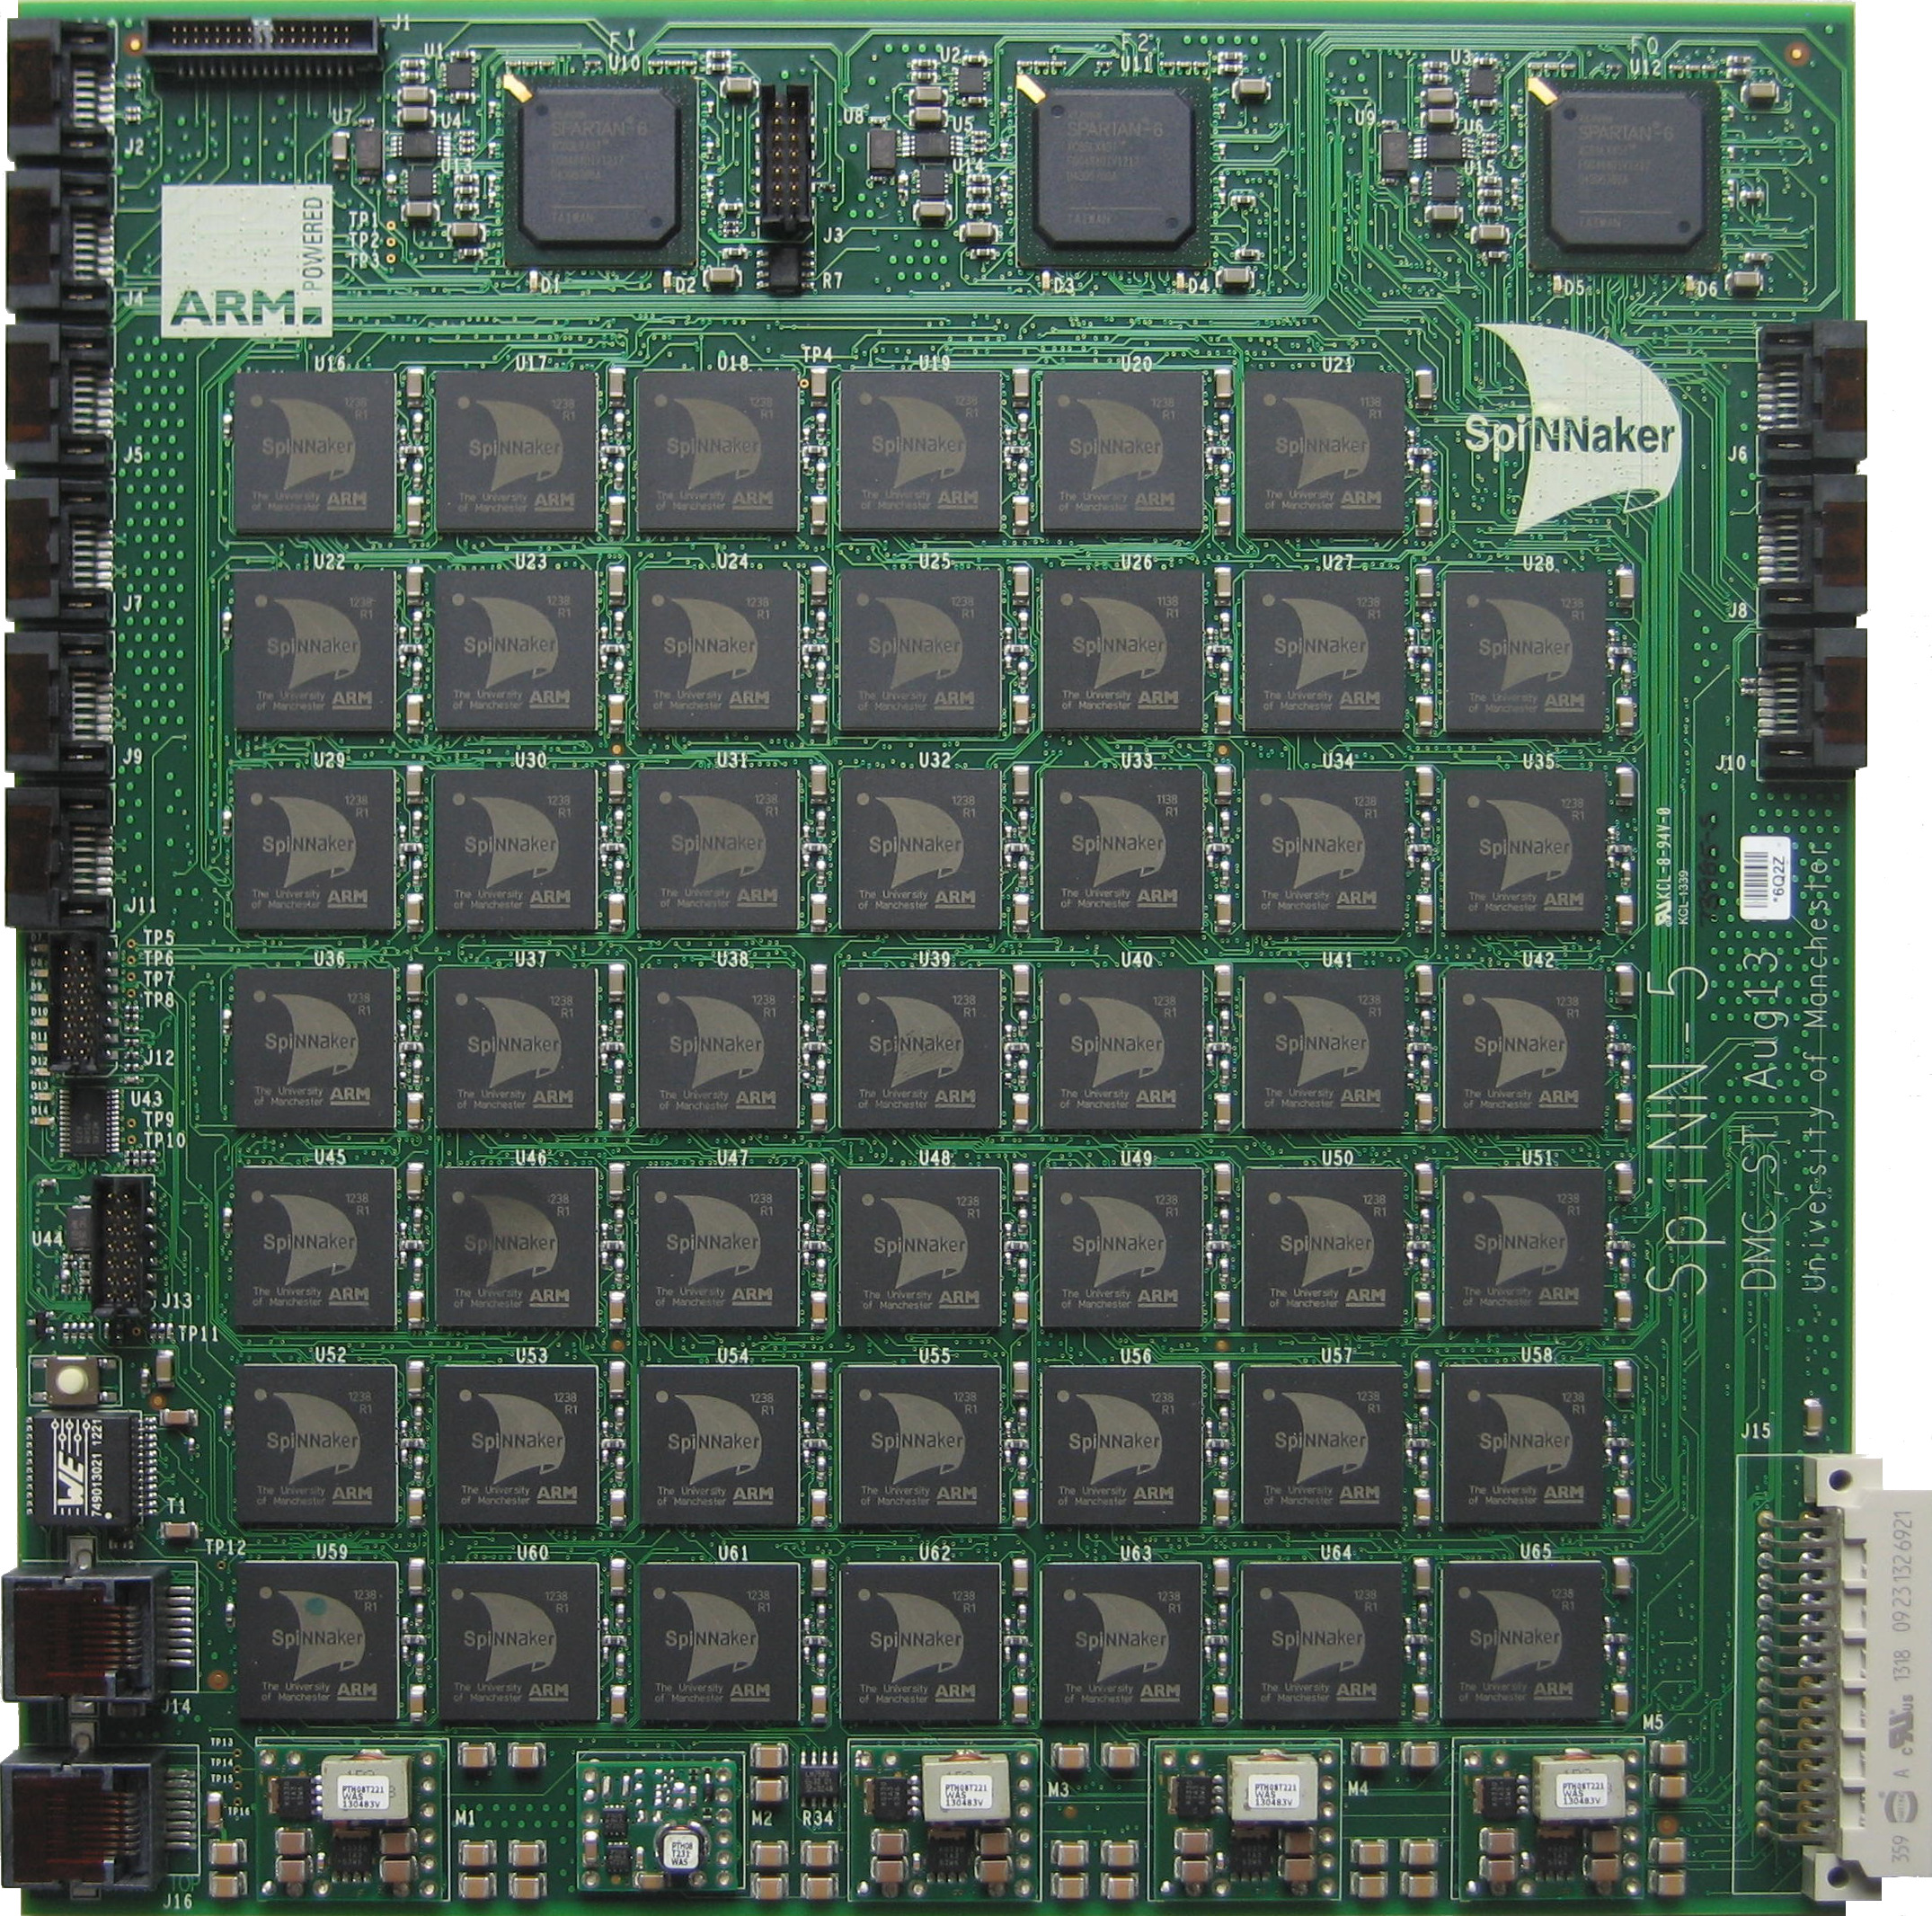
\includegraphics[width=0.45\linewidth]{images/spin5.jpg}
	\caption{48-chip SpiNNaker board.}
	\label{fig:spin5}
\end{figure}

\subsection{Hardware fault tolerance mechanisms}
The SpiNNaker chip has been designed with fault tolerance in mind. The SpiNNaker chip is made up of various blocks, most of which have a certain degree of hardware fault tolerance in place. The blocks in being considered are: the ARM968, the Vector Interrupt Controller (VIC), the counter/timer, the DMA controller, the communications controller, the router, the inter-chip transmit and receiver interfaces, the SDRAM interface, the Ethernet interface, the system RAM and the boot ROM. A schematic representation of all these sub systems is shown in \textbf{Figure~\ref{fig:spin_arch}}.

\subsubsection{Block description}
\begin{itemize}
	\setlength\itemsep{2pt}
	\item The \textbf{ARM968} together with the tightly-coupled instruction and data memories, form the core processing resource in SpiNNaker.
	\item Each processor node on an SpiNNaker chip has a \textbf{Vectored Interrupt Controller} (VIC) that is used to enable  and disable  interrupts  from  various  sources,  and  to wake  the processor  from  sleep mode when required.
	\item Each processor node has a \textbf{Counter/Timer}.
	\item Each ARM968 processing subsystem includes a \textbf{DMA controller}. The DMA controller is primarily used for transferring inter-neural connection data from the SDRAM in large blocks in response to an  input  event  arriving  at a  fascicle processor, and  for  returning updated connection data during learning. In addition, the DMA controller can transfer data to/from other targets on the System NoC such as the System RAM and Boot ROM.
	\item	Each processor node on SpiNNaker includes a \textbf{Communications Controller} which is responsible for generating and receiving packets to and from the communications network.
	\item The \textbf{Router} is responsible for routing all packets that arrive at its input to one or more of its outputs. It  is  responsible  for  routing multicast neural event packets, which  it does  through an associative multicast  router  subsystem,  point-to-point  packets  (for  which  it  uses  a  look-up  table),  nearest-neighbour packets  (using  a  simple  algorithmic process),  fixed-route packet  routing  (defined  in  a register), default routing (when a multicast packet does not match any entry in the multicast router) and emergency routing (when an output link is blocked due to congestion or hardware failure). Various error conditions are identified and handled by the Router, for example packet parity errors, time-out, and output link failure.
	\item \textbf{Inter-chip  communication}  is  implemented  by  extending  the Communications NoC  from  chip  to chip.  In  order  to  sustain  throughput,  there  is  a  protocol  conversion  at  each  chip  boundary  from standard CHAIN 3-of-6 return-to-zero to 2-of-7 non-return-to-zero. The interfaces include logic to minimise the risk of a protocol deadlock caused by glitches on the inter-chip wires.
	\item The \textbf{SDRAM  interface}  connects  the System NoC  to  an off-chip SDRAM device.
	\item \textbf{Ethernet interface} --- The  SpiNNaker  system  connects  to  a  host  machine  via  Ethernet  links.  Each  SpiNNaker  chip includes  an  Ethernet MII  interface with the interface hardware operating at the frame level. All higher-level protocols are implemented in software running on the local monitor processor.
	\item The \textbf{System RAM} is an additional 32~kB block of on-chip RAM used primarily by the monitor processor to enhance its program and data memory resources as it will be running more complex (though less time-critical) algorithms than the fascicle processors. As the choice of monitor processor is made at start-up (and may change during run-time for fault-tolerance  purposes)  the  system  RAM  is  made  available  to  whichever  processor  is  monitor processor via  the System NoC. Accesses by  the monitor processor  to  the System RAM are non-blocking as far as SDRAM accesses by the fascicle processors are concerned. The System RAM may also be used by  the fascicle processors to communicate with  the monitor processor and with each other, should the need arise.
	\item The \textbf{Boot ROM} consists of a 32~kB on-chip ROM to provide minimal support for initial self-test and monitor processor selection. It also provides support for router initialisation for bootstrapping and system boot.
\end{itemize}

\begin{figure}[t]
	\centering
	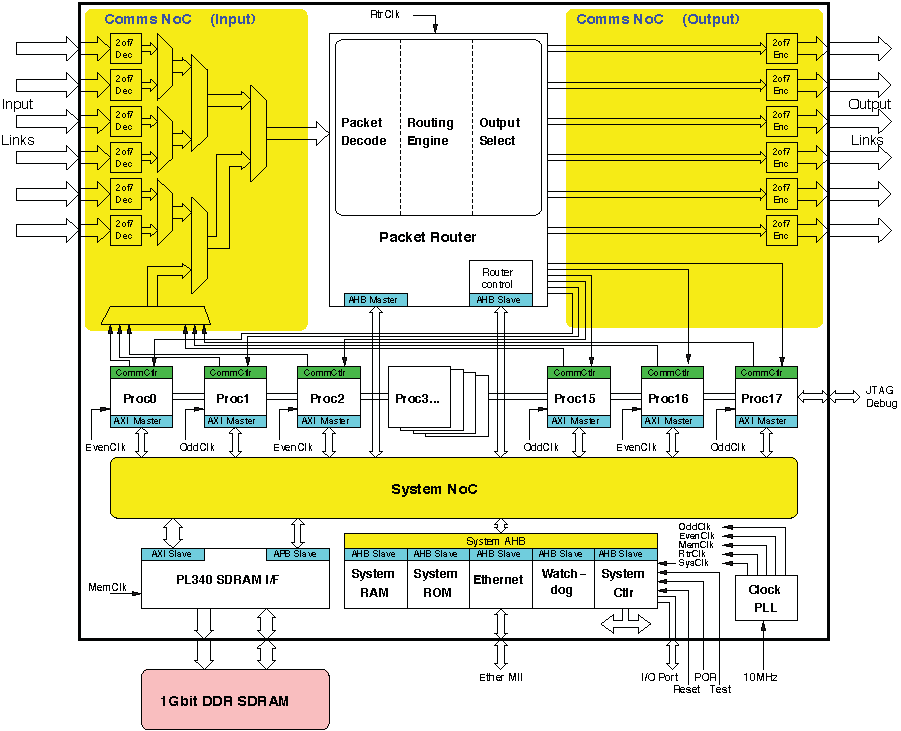
\includegraphics[width=0.65\linewidth]{images/spinnaker_architecture.pdf}
	\caption{SpiNNaker chip subsystems.}	
	\label{fig:spin_arch}
\end{figure}

\subsubsection{Possible fault tolerance mechanisms}
This section outlines the various blocks in the SpiNNaker chip which could potentially be used to implement a robust fault tolerant system. At the time of writing, only the router, the vector interrupt controller and the CRC unit are being effectively used to provide a certain level of fault tolerance.

The \textbf{ARM968} processor core (\textbf{Figure~\ref{fig:arm968}}) has self-test routines that are run at start-up and during normal operation to provide a fault tolerance detection mechanism and a chip-wide watchdog timer catches runaway software. In addition, the ARM968 is able to isolate defective instruction and data RAM locations and can be mapped out by software. The system controller can also disable any incorrectly operating ARM968 cores. These detection and fault isolation mechanisms help to reconfigure the system in case a fault is detected. In the case of faulty instruction and data RAM, software can be written to avoid such locations. If on the other hand, the self-test and start-up routines detect a failure, the processor core functionality can be migrated to a neighbouring processor (see \textbf{Section~\ref{sec:migration}}).

Currently the \textbf{vector interrupt controller} does not provide a high degree of fault tolerance. In the case of a failed vector location, the vector interrupt controller effectively jumps to a random location. If a software mechanism was devised to detect these kind of faults, a failed vector location could be removed from service (provided there are enough vector locations available). Another solution would be to shut down the entire vector system and the interrupts run by software inspection of the IRQ status registers.

In order to detect faults in the \textbf{counter/timer}, the second counter/timer could be configured with a longer period to check the calibration of the first. Assuming that the system only requires one counter/timer, and a fault is detected, the faulty counter could be disabled, with the operational counter/timer taking over.

\begin{figure}[t]
	\centering
	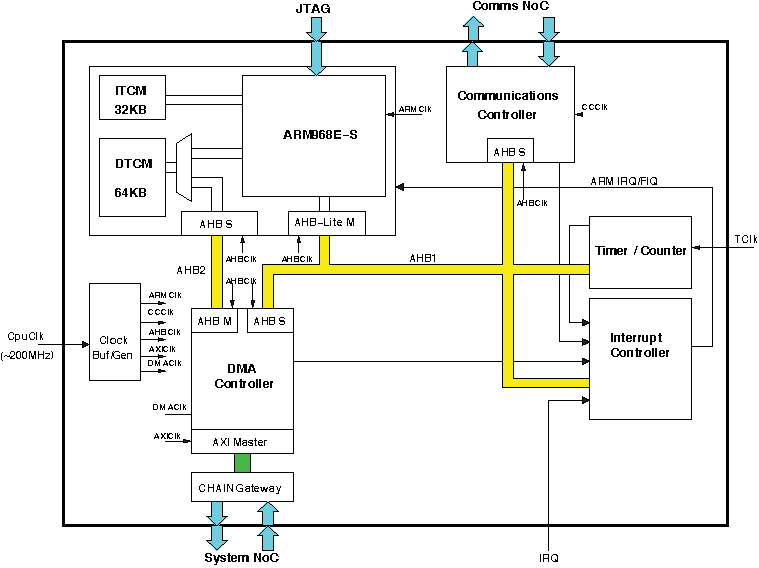
\includegraphics[width=0.55\linewidth]{images/arm968_subsystem.pdf}
	\caption{ARM 968 subsystem.}
	\label{fig:arm968}
\end{figure}

The \textbf{DMA controller} has a CRC unit (more on this in \textbf{Section \ref{sec:crc}}) which can be used to detect errors in the data transferred by the DMA controller. If an error is detected by means of the CRC unit, the data block could be retransmitted. The DMA controller will also time-out if a transaction takes too long. If if the error rate is consistently high, fault tolerant software could be written to shut down the local processing subsystem and its functions migrated to another subsystem on the current or to another chip.

The \textbf{communications controller} is able to detect the following kinds of faults:
parity of received packet, received packet framing error, and transmit buffer overrun. Since the communications controller is mission-critical to the local processing subsystem, it should be disabled and isolated and its functions migrated to another subsystem on the current or onto another chip if a failure is detected.

The \textbf{router} is a complex piece of circuitry and is endowed with some internal fault-tolerance capacity. In particular it is possible to map out a failed multicast router entry --- useful since the multicast router dominates the silicon area of the communications router. It also has the capacity to cope with external failures. Emergency routing will attempt to bypass a faulty or blocked link. In the event of a node (or larger) failure this will not be sufficient and in order to tolerate a chip failure several measures can be employed on a local basis:
\begin{itmz}
	\item Point-to-point packets can be routed around the obstruction,
	\item Multicast packets with a router entry can be redirected appropriately.
\end{itmz}
In most cases, default multicast packets cannot sensibly be trapped by adding table entries due to their (almost) infinite variety. To allow re-routing, these packets can be dropped to the monitor processor on a link-by-link basis using the diversion register. In principle they can then be routed around the obstruction as point-to-point payloads before being resurrected at the opposite side. Should the monitor processor become overwhelmed, it is also possible to use the diversion register to eliminate these packets in the router; this prevents them blocking the router pipeline while waiting for a time-out and thus delaying viable traffic.

The router is able to detect a variety of faults, namely: packet parity errors, packet time-phase errors, packet unroutable errors, and wrong packet length. In the case any of the above faults are detected, a multicast router entry can be disabled. The router can also be reconfigured to get around certain faults, e.g., since all multicast router entries are identical, the function of any entry can be relocated to a spare entry. Also, if a router becomes full, a global reallocation of resources can move functionality to a different router.

The \textbf{inter-chip transmit and receive interfaces} (see \textbf{Figure~\ref{fig:interchip_links}}) can be made robust to faults by having the monitor process regularly test the link functionality. If a fault is detected the link interface can be reset by the system controller to attempt recovery from the fault, and the link interface can be isolated and an alternative route used. The interfaces are `glitch hardened' to greatly reduce the probability of a link deadlock arising as a result of a glitch on one of the inter-chip wires. Such a glitch may introduce packet errors, which will be detected and handled elsewhere, but it is very unlikely to cause deadlock.

The \textbf{SDRAM interface} is endowed with Delay-Locked Loop (DLL) delay lines (including a spare) which can be tested for stuck-at faults and relative timing accuracy. If a fault in the timing is detected, the SDRAM interface can be isolated and replaced by using the spare delay line.

The \textbf{Ethernet MII interface} is only used in a small number of nodes, specifically one for each group of 48 chips and thus most nodes are insensitive to faults in its functionality as they will not attempt to use it.

To detect faults in the \textbf{system RAM}, the monitor processor could perform a system RAM test at start-up, and also periodically during the course of the system operation. Since the system RAM does not employ any kind of parity or ECC system, it is not clear how soft errors can be detected. If an error is detected during the start-up test, faulty words could be mapped out of use. If the system RAM is deemed unusable, the only other option (short of completely disabling the entire chip) would be to use the SDRAM instead. This will probably result in compromised performance for the fascicle processors due to loss of SDRAM bandwidth.

A fault in the \textbf{boot ROM} can be easily detected during start-up if the boot ROM fails the boot process. One can easily switch the boot ROM out of the boot area rendering it harmless. When the boot ROM is switched out of the boot area the system RAM is switched in the boot area and a neighbouring chip can initialise the system RAM with the boot code and retry initialisation.

\begin{figure}[b]
	\centering
	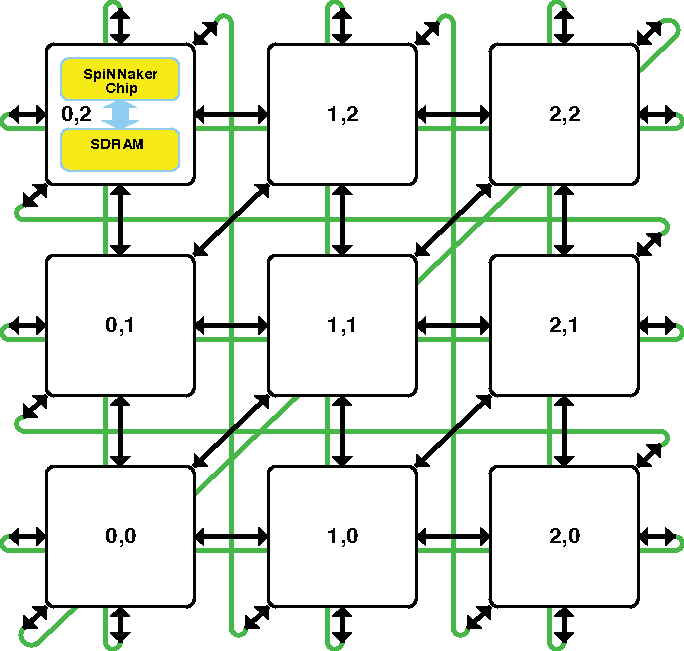
\includegraphics[width=0.35\linewidth]{images/system_architecture.pdf}
	\caption{SpiNNaker inter-chip links.}
	\label{fig:interchip_links}	
\end{figure}

\clearpage
\section{Network congestion}
\label{sec:congestion}

\subsection{Dumped-packet reinsertion}

%\verb|dumpBounce.c|:  packet re-injection software that runs on a separate core.
 
\emph{Network Tester} is a library designed to enable experimenters to quickly and easily describe and run experiments on SpiNNaker's interconnection network \citep{heathcote2015networktester}. \hl{is dumpBounce.c somehow used?}. \emph{Network Tester} makes use of \verb|dumpBounce.c| developed by Luis A. Plana which is the packet re-injection `brains' that runs on a separate application core. In particular, \emph{Network Tester} is designed to make recreating traffic loads similar to typical neural software straight-forward. Such network loads feature a fixed set of vertices (cores) that produce SpiNNaker packets which are then multicast to a fixed set of vertices. The following is a list of the kinds of experiments which can be performed with \emph{Network Tester}:
\begin{itemize}
\item Determine how a network copes with different rates and patterns of packet generation, in order to determine the maximum speed at which a particular neural simulation may run on SpiNNaker without dropping packets;
\item Determining the effectiveness of place and route algorithms by finding `hot-spots' in the network;
\item Characterising the behaviour of the network in the presence of locally and globally synchronised bursting traffic.
\end{itemize}

\subsection{Results}
\begin{figure}[h]
	\begin{subfigure}{.5\linewidth}
		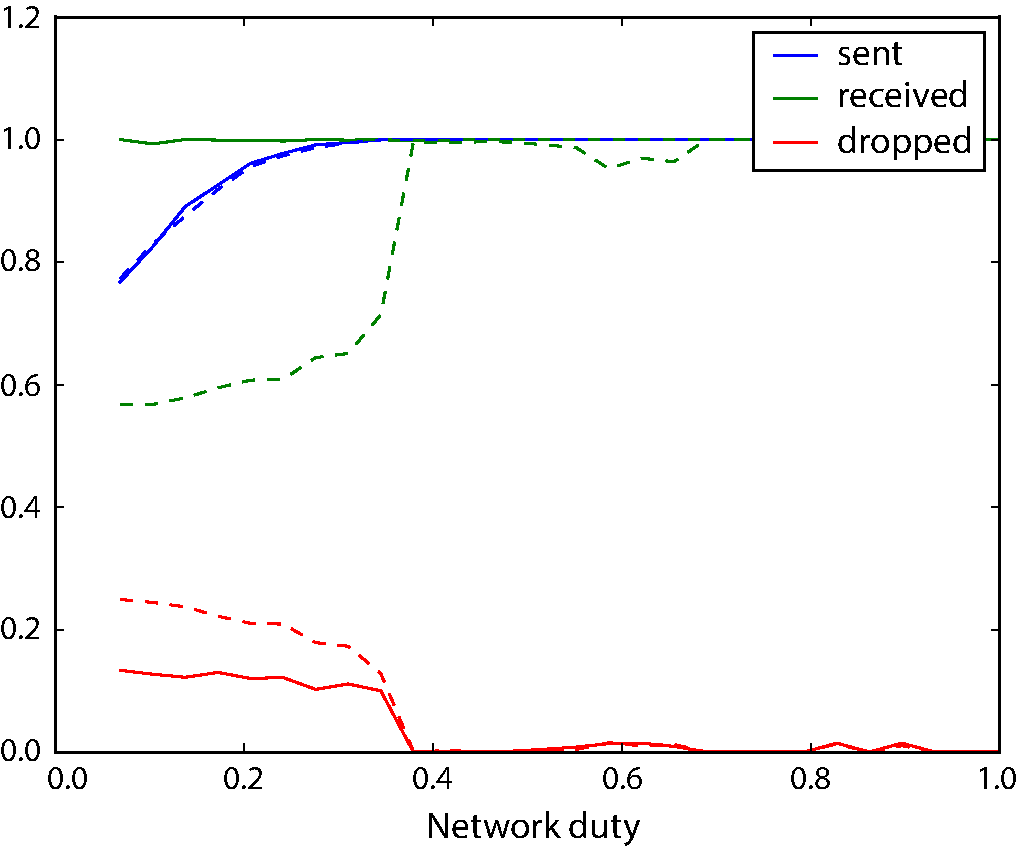
\includegraphics[width=0.9\linewidth]{images/bursting.pdf}
		\caption{Bursting}
		\label{fig:bursting}
	\end{subfigure}
	\begin{subfigure}{.5\linewidth}
		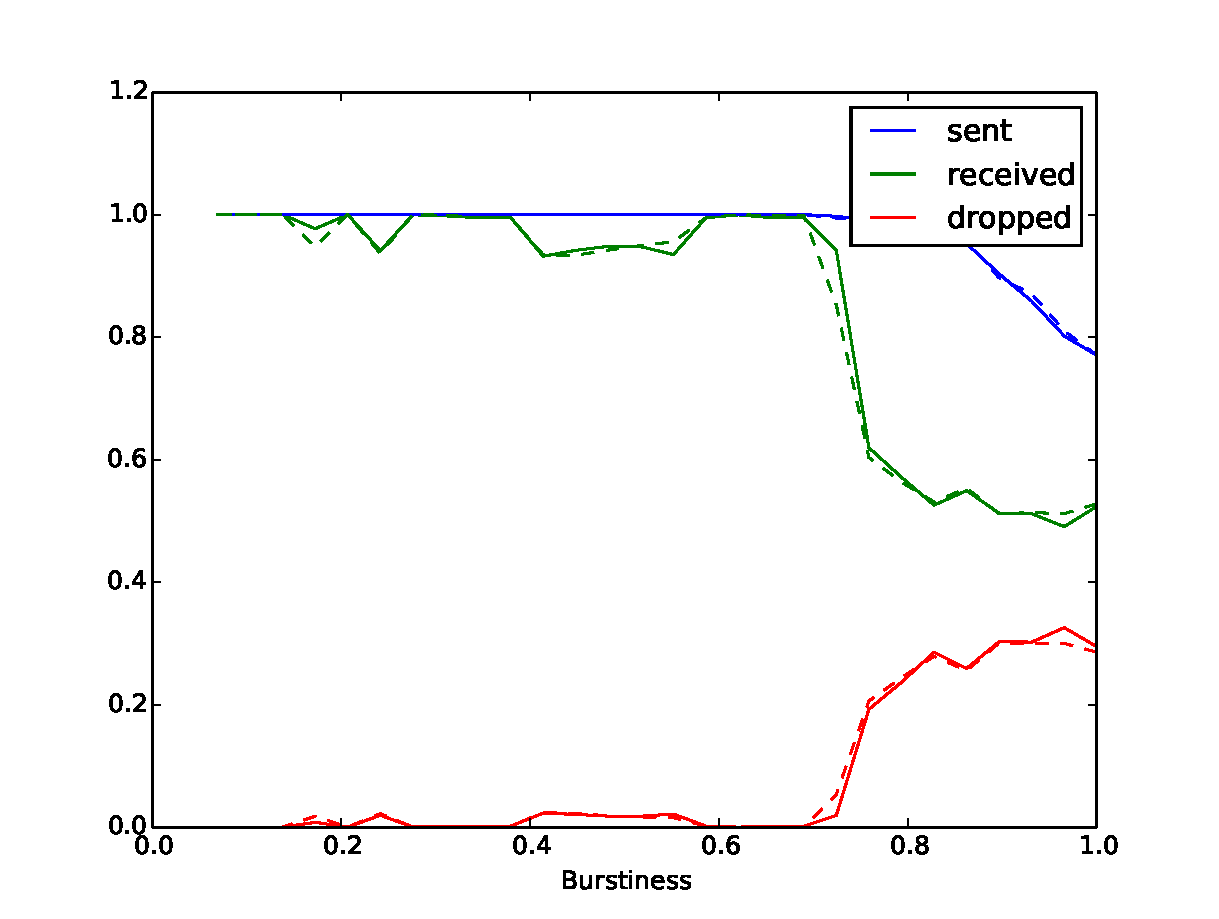
\includegraphics[width=0.9\linewidth]{images/bursting_connaware2.pdf}
		\caption{Bursting (connection-aware)}	
		\label{fig:bursting_aware}
	\end{subfigure}
	\caption{Network congestion with respect to network load.}
\end{figure}

Clearly with packet reinjection, nearly all packets which are actually sent arrive at their destination, without reinjection, things aren't so great.

Fun things to try: Uncomment lines 23--24 and the random network will get placed by what PACMAN calls ``connectivity-aware placement,'' rather than simulated annealing (the default). Interestingly, on my system this results in reinjection no-longer helping and the whole thing being even worse under bursty packets.

\begin{figure}[htbp]
	\centering
	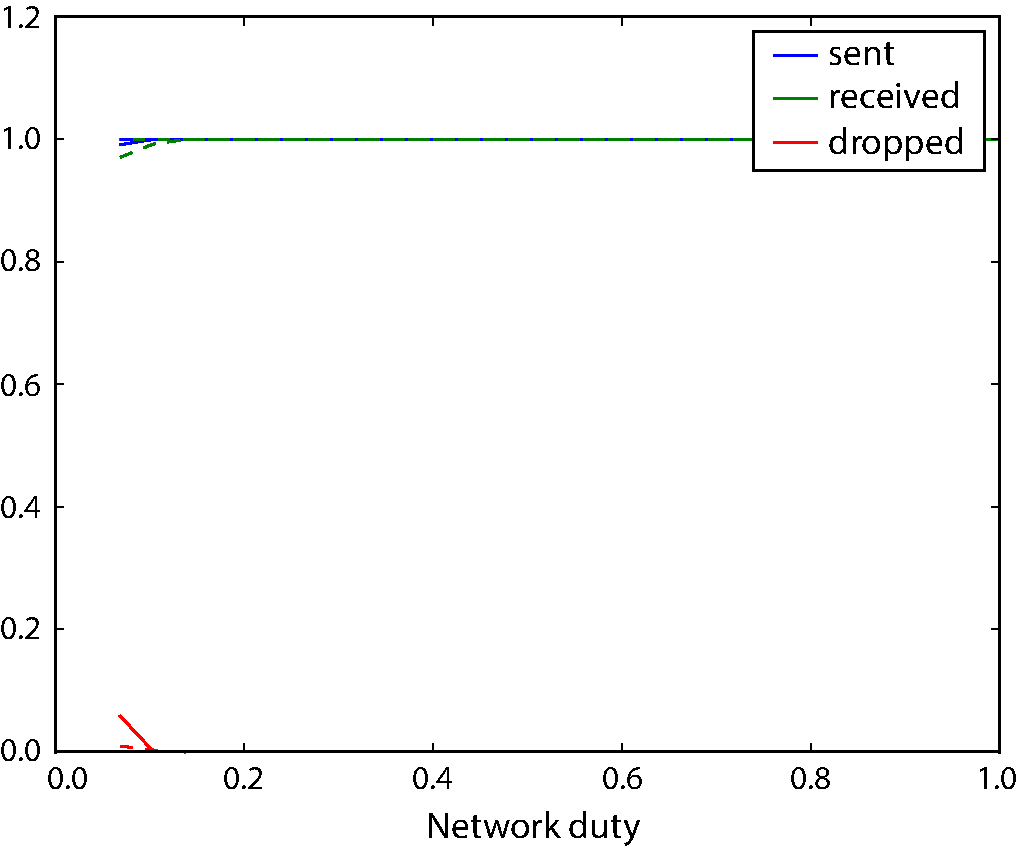
\includegraphics[width=0.5\linewidth]{images/bursting_random.pdf}
	\caption{Network congestion in a bursty (random) situation.}	
	\label{fig:bursting_random}
\end{figure}

Add the line \verb|e.burst_phase = None| somewhere before \verb|e.run()| is called and the packet generators will still generate bursts but they'll be at random phases to each other (i.e., not bursting all at the same time). This normally eliminates packet dropping for all but the most extreme burstiness.

\begin{enumerate}
\item Backpressure during the first bit (blue 0--0.4) resulting in a lower number of packets sent
\item Important line is green (true measure of whether packets are being dropped or not)
\item Number of packets sent is constant for every point (=32) along the x-axis. Network duty=0.1 means that all the packets are sent in 0.1*1ms, i.e. in a very short period of time, i.e. high network load. Network duty=1 means that the whole 1 ms is used to transmit all of the 32 packets.
\item Dropped packets (solid red) are dropped but reinjected so not really dumped vs the dashed red line where packets are dropped and dumped.
\item Packets sent is the same in every point calculated, only the level of bursting is changed.
\item Same colour curves share the same axis scale.
\item (a) uses simulated annealing ("smarter"), (b) dumb placement as that used in PACMAN
\end{enumerate}

\clearpage
\section{Process migration}
\label{sec:migration}

Process migration work in SpiNNaker is currently being implemented in the \emph{heat demo} demonstration program. The \emph{heat demo} (developed by Luis A. Plana) is an ideal environment to test process migration experiments because it consists of the computation of a set of highly parallel finite difference equations which produce reliable and repeatable results. This is in contrast to spiking neural network simulations which due to the random nature of the input spikes as well as the numerical errors that might creep in while computing the neuron differential equations, make them a poor choice for testing out different function or process migration schemes. 

Two versions of the \emph{heat demo} are available:
\begin{itemize}
\item \verb|heat_demo_ft.c| is a version with basic function migration capability where the \emph{leadAp} core, i.e., the core which has been assigned as the primary core out of the 16 application cores will take out a non-working core and takes over its functionality. This is done by stripping the broken cores from the routing entries. This process can be repeated till there are no more available working application cores. \verb|heat_demo_ft.c| is currently not able to deal with a crashed \emph{leadAp} core and in this case function migration will not take place.

\item \verb|heat_demo_bt.c| tries to solve the problem of a broken \emph{leadAp} core by replacing it with a working application core. The strategy is slightly different from the one implemented in \verb|heat_demo_ft.c|, but simpler to implement since all the \hl{cores poll at the same frequency}. In this case, a broken core is simply taken out from the routing entries and no function migration takes place.
\end{itemize}

\subsection{Background}
The heat demo is essentially a 2D heat diffusion equation solver. The heat equation is a partial differential equation that describes the variation in temperature over time in a region, given an initial temperature distribution and the boundary conditions. For a temperature $u(x,y,t)$ of two spatial variables $x$ and $y$ and the time variable $t$, the 2D heat equation is:
\[
\dpd{u}{t} -\alpha\left( \dpd[2]{u}{x} + \dpd[2]{u}{y} \right) = 0 
\]
where $\alpha$ is the thermal diffusivity, a material-dependent positive constant. A common way to solve this equation numerically is to approximate the derivatives by finite differences, generating a finite-difference discretisation of the heat equation.

Relaxation methods are iterative numerical methods used to solve systems of equations, including non-linear systems. In particular, they are commonly used to solve finite-difference discretisations of differential equations, such as the heat equation. A time-stepping algorithm is used to compute the new temperature of each point in the region, based on its current temperature and that of its neighbouring points:

\begin{align*}
\Delta x   &= \beta_x \cdot [u(x+1,y,t) + u(x-1,y,t) - 2 \cdot u(x,y,t)] \\
\Delta x   &= \beta_y \cdot [u(x,y+1,t) + u(x,y-1,t) - 2 \cdot u(x,y,t)] \\
u(x,y,t+1) &= u(x,y,t) + \Delta x + \Delta y
\end{align*}

%\noindent A visualisation of the above equations is depicated in \textbf{Figure~{\ref{fig:heatdemo_iterative}}}.
%\begin{figure}[htbp]
%	\centering
%	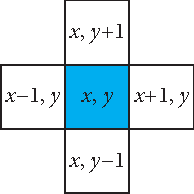
\includegraphics[width=0.15\linewidth]{images/heatdemo_finitediff.pdf}
%	\caption{2D heat diffusion --- finite difference method.}	
%	\label{fig:heatdemo_iterative}
%\end{figure}

These methods are well-suited for parallel implementation following a Single Program, Multiple Data (SPMD) model in which multiple autonomous cores simultaneously execute the same program with different data, and use messages to communicate with each other. In the heat equation case, each point sends its temperature to four neighbours and receives their temperatures in each time step. Using a relaxation method to solve the heat equation is easily and efficiently mapped to SpiNNaker. In particular, the communications pattern is that which SpiNNaker is optimised for: many short messages sent concurrently to several destinations.

To implement the algorithm in SpiNNaker, the entire region is partitioned into sub-arrays of points and distributed across the machine. In the extreme case, every core is assigned a single point. Each core can then compute the corresponding temperatures and distribute them to its neighbours using SpiNNaker's efficient multicast communication infrastructure.

In the case of \verb|heat_demo_ft.c|, if a broken core is detected the \emph{leadAp} core takes over its function with the result that two points are now computed on one core. Since the calculation of one point is very simple this doesn't result in an appreciable increase on the CPU load and the application is not slowed down. In more compute-intensive applications this might result in bottlenecks.

In SpiNNaker, the topology of the problem is dissociated from the topology of the machine, i.e., the mapping of points to cores in SpiNNaker is completely flexible and neighbouring points may not be mapped to neighbouring chips. Once the routing tables have been setup by the programme, a core can send a message with its current temperature and the communications infrastructure is responsible for the delivery of that message to the correct places.

SpiNNaker promotes event-driven software: cores respond to events and carry out the necessary computations. In the mean time, the cores are in low-power mode to save energy. Polling and idle iterations are avoided. In the heat equation solver, the arrival of a neighbour's temperature and the lapse of the time interval will trigger a core into operation.

\begin{figure}[htbp]
	\centering
	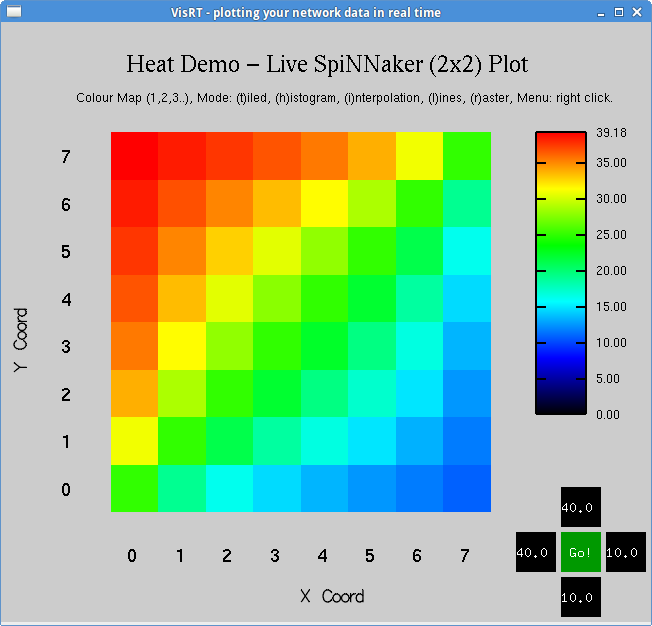
\includegraphics[width=0.6\linewidth]{images/heatmap2x2.png}
	\caption{Heat map demo visualisation on a 4-chip SpiNNaker board.}
	\label{fig:heatmap}
\end{figure}

\textbf{Figure~\ref{fig:heatmap}} shows a snapshot of the output visualizer of a 2D heat diffusion solver running on a 64-core (4-chip) SpiNNaker board. In this example, each of the 64 application cores in SpiNNaker is assigned a single point in a ``hexagonal'' region. Each square in the plot represents the temperature at a given point in the region.

%The user can control the temperatures of the North, South, East and West boundaries and view the evolution of temperatures over time. The figure shows a scenario in which the North and West boundaries have been set to 40~\textdegree C and the East and South boundaries to 10~\textdegree C.
%
%To test out the \verb|heat_demo_ft| functionality, start the \verb|heat_demo_ft.aplx|
%by running (from ybug) \verb|@ heat_demo_ft_1board.ybug|
%
%Then start resetting cores one-by-one by writing directly to the system
%controller register \verb|(0xe2000000:r1 = 0xe2000004)|\\
%Command: \verb|sw 0xe2000004 0x5ec00002|
%
%Note: If the core you reset happens to be the leadAp, the application will
%crash.
%
%\emph{Currently implemented on the heat demo, where a core fault is simulated by intentionally reset a core. Currently if core 1 on core (0,0) is reset or disabled no communication is possible with the host PC.}


\clearpage
\section{CRC error correction}
\label{sec:crc}

The preservation of digital data integrity is of major concern for computer, communication, and storage systems. In all these applications digital data is susceptible to unintentional modification which may arise from electrical or magnetic disturbance, component failure, or the result of system design error. Depending on the specific application, data failures may result in severe consequences and thus their potential occurrence needs to be considered carefully in the underlying design of the system.

Data reliability can be enhanced through the employment of error-control codes,which provide mechanisms for the detection and correction of errors. These codes enrich the data with redundancy by forming code words, which initially can be used to detect inconsistencies in the received data. If the affected data can be retransmitted or recalculated, one simple error correction scheme is the Automatic Repeat Query (ARQ), where the receiver simply requests a retransmission once it detects data inconsistencies. However, where retransmission or recalculation is not feasible, being too slow or uneconomic, Forward Error Correction (FEC) techniques can correct errors on the basis of the corrupted received data and its inherent redundancy.

Cyclic codes form an important class of error-control code offering powerful error detection and correction capabilities. At the same time, their algebraic properties permit the use of simplified processing procedures when compared to non-cyclic codes. For instance, the encoding of data into cyclic code words can easily be achieved in hardware using a simple linear feedback shift register. Likewise, the same circuit can be used to validate code words, and thus detect errors. For these reasons, cyclic codes have been widely adopted as error-detecting codes and commonly deployed in combination with ARQ schemes \citep{grymel2013error}. 

If error correction is desired, the most basic case concerns the localisation of a single erroneous bit. It can be shown that for cyclic codes this problem is equivalent to the computation of the discrete logarithm in finite cyclic groups, for which it is widely believed that for the general case no efficient classical algorithm is devisable. However, it has not been proven that the computation of the discrete logarithm is hard for all groups of practical interest \citep{grymel2013error}.

Cyclic codes are characterised by an underlying generator polynomial. Different generator polynomials exhibit different capabilities in regard to the detection and correction of errors. Certain polynomials, for example, may be particularly well suited to the practical realisation of the error correction process. The selection of polynomial is also dependent on the length of the data that is to be protected and the anticipated error patterns. In systems where diverse applications may favour different cyclic codes, and where the requirements may change over time or be unknown at the design stage, it may be advantageous to provide full flexibility in regard to the usable cyclic code generator polynomials. SpiNNaker employs programmable cyclic code circuits to enable the efficient processing of cyclic codes.

\subsection{Discrete logarithms}
In mathematics, a discrete logarithm is an integer $k$ solving the equation $b^k = g$, where $b$ and $g$ are elements of a finite group. Discrete logarithms are thus the finite-group-theoretic analogue of ordinary logarithms, which solve the same equation for real numbers $b$ and $g$, where $b$ is the base of the logarithm and $g$ is the value whose logarithm is being taken \citep{wiki:discretelogs}.

No efficient classical algorithm for computing general discrete logarithms $\log _b g$ is known. The naive algorithm is to raise $b$ to higher and higher powers $k$ until the desired $g$ is found. This algorithm requires running time linear in the size of the group $G$ and thus exponential in the number of digits in the size of the group.

More sophisticated algorithms exist, usually inspired by similar algorithms for integer factorization. These algorithms run faster than the naive algorithm, some of them linear in the square root of the size of the group, and thus exponential in half the number of digits in the size of the group. However, none of them run in polynomial time.

\subsection{Memory faults}
The large SpiNNaker system in its envisaged configuration of 57,600 nodes will incorporate approximately 7~TB of SDRAM. With such an immense amount of memory, the effect of data bit errors is significant during the operation of the machine.

Memory bit errors are subdivided into two different classes: hard and soft errors. A hard error is characterised by a permanent hardware fault in a memory cell that will result in a consistent reliability issue. For instance, it may be the case that a memory cell will always provide one particular bit value during readout, no matter what value has been written to it. Soft errors are transient faults that occur randomly and may, for example, be induced through cosmic rays or the decay of radioactive atoms in the memory packaging materials. Also, a soft error may arise either directly in the memory, or along the data path during the memory read or write phase.

Recently, a large-scale study has been conducted to investigate statistics for error rates in Dynamic Random Access Memory (DRAM) in production systems \citep{schroeder2009dram}. It suggests that the average error rate ranges from 25,000 to 75,000 FIT (failures in time per billion hours of operation) per Mbit, however a distinction between hard and soft errors is not made. If these numbers are applied to the SpiNNaker system of 57,600 nodes, 25 to 74 bit errors on average can be expected to occur within the SDRAM per minute, roughly approximated as one bit error per second.

It may be the case that the number of expected bit errors in the SpiNNaker system will not have a significant impact on particular applications such as neural network simulations. However, it is not known to what extent neural network simulations can compensate for memory faults, and other potential applications may not tolerate bit errors at all, so appropriate measures need to be taken to deal with them in the SpiNNaker system. For this reason error-control codes are employed within SpiNNaker to provide a layer of protection against memory faults.

\subsection{CRC unit}
The DMA controller of each processing subsystem in SpiNNaker is equipped with a CRC unit that allows the generation and verification of error-control codes. The circuit primarily supports cyclic codes as they offer powerful error detection and correction capabilities and because they are easily implementable in hardware \citep{costello2004error}. Programmable cyclic code circuits have the benefit of flexible adaptation of the underlying cyclic code to meet the requirements of a specific application. The main drawback of cyclic codes is the lack of efficient error correction techniques. To perform the correction of a single-bit error an instance of the generalised discrete logarithm problem needs to be solved.

If, for instance, a processor initiates a DMA transfer to copy a data block from the local memory to the SDRAM, the CRC unit can be instructed to calculate (transparently and in parallel) the redundancy part for a cyclic code and, automatically, append this to the SDRAM data block. The CRC unit can be used to calculate the error syndrome for a data block retrieved from memory and signal the corresponding processing core if an integrity issue arose. The program that is executed on the processing core has to decide what action is to be taken in the event of a detected data inconsistency. A simple retransmission of the data block could correct the error if it occurred along the data path during the readout phase, however even this may not be fast enough for the `real-time' operation of a SpiNNaker neural simulation. Therefore it is necessary to consider appropriate error correction procedures in software, to recover from memory faults based on the obtained error syndrome, including when they are uncorrectable. These can range from a simple disregard of the error, through a localisation and correction of the error, to a shutdown of the relevant SpiNNaker system components for replacement if hard errors are involved.

In the choice of employed cyclic code, many factors need to be taken into account for the selection of the generator polynomial. For instance, certain undiscovered subclasses of cyclic codes may allow the realisation of very efficient error correction procedures in software, or data blocks of different lengths may be stored in the SDRAM so that a polynomial offering best combined error protection for all of the block lengths should be selected. The programmable CRC circuit in SpiNNaker permits switching the generator polynomial to any of degree 32 or lower whenever required. A direct advantage is that the polynomial is adaptable to the length of the data block that is to be protected, which means that the best choice of offered error protection can be made. Another feature of the CRC circuit is that several cyclic codes of a smaller degree can be generated based on different bits of the data stream. For example, for each half-word of the data stream, a cyclic code based on a generator polynomial of degree 16 can be computed.

\subsection{Algorithms for Computing Discrete Logarithms}
\citet{grymel2013error} developed two new approaches for computing discrete logarithms to facilitate the correction of single-bit errors based on cyclic codes. The first approach is generic in nature leading to a deterministic algorithm for group orders that equal a Mersenne number with an exponent of a power of two; this algorithm has constant space requirements and runs in the worst case in the order of the square root of the group order. It was shown how the algorithm can be improved if the discrete logarithm values occur with unequal probabilities and that certain properties hold for the associated sequences. The second approach for the computation of discrete logarithms is based on a subset of newly developed properties for finite fields of binary characteristic represented as the polynomial ring over the binary field modulo a primitive polynomial. For evaluated small fields, a deterministic efficient algorithm with linear space and linearithmic time requirements in the degree of the defining polynomial was devised.

\newpage
\begin{appendices}

\section{Code listings}
\usemintedstyle{vs}
%\captionof{listing}{dumpBounce.c}
%\begin{multicols}{2}
%\inputminted[fontsize=\tiny]{c}{code/dumpBounce.c}
%\end{multicols}
%
%\clearpage
%\captionof{listing}{backpressure.py}
%\begin{multicols}{2}
%\inputminted[fontsize=\tiny]{python}{code/backpressure.py}
%\end{multicols}
%
\captionof{listing}{bursting.py}
\begin{multicols}{2}
\inputminted[fontsize=\tiny]{python}{code/bursting.py}
\end{multicols}
\end{appendices}

\newpage
\bibliographystyle{abbrvnat}
\bibliography{fault_tolerance_report}
\end{document}
